% This is samplepaper.tex, a sample chapter demonstrating the
% LLNCS macro package for Springer Computer Science proceedings;
% Version 2.20 of 2017/10/04
%
\documentclass[runningheads]{llncs}
%
\usepackage[utf8]{inputenc}
\usepackage{amsmath}
\usepackage{tikz}
\usetikzlibrary{automata,positioning}
\usepackage{amssymb}
\usepackage{caption}
\usepackage{subcaption}
\usepackage{float}
\usepackage{wrapfig}
\usepackage{graphicx}
\usepackage{todonotes} 
\usepackage{hyperref}
\usepackage{float}
\restylefloat{table}
\usepackage{tikz}
\usepackage{wrapfig}
\usetikzlibrary{shapes, arrows}
% Used for displaying a sample figure. If possible, figure files should
% be included in EPS format.
%
% If you use the hyperref package, please uncomment the following line
% to display URLs in blue roman font according to Springer's eBook style:
% \renewcommand\UrlFont{\color{blue}\rmfamily}

\begin{document}
%
\title{Measuring the quality of ontology matches in BioPortal}
%
%\titlerunning{Abbreviated paper title}
% If the paper title is too long for the running head, you can set
% an abbreviated paper title here
%
\author{Tobias R\"awer \and
Lina Molinas Comet \and
Jonas R\"ulfing}
%
\authorrunning{R\"awer et al.}
% First names are abbreviated in the running head.
% If there are more than two authors, 'et al.' is used.
%
\institute{RWTH Aachen University, Aachen, Germany 
\email{\{tobias.raewer,lina.molinas.comet,jonas.ruelfing\}@rwth-aachen.de}\\
\url{http://dbis.rwth-aachen.de/cms}}
%
\maketitle              % typeset the header of the contribution
%
\begin{abstract} \label{abstract}
BioPortal \footnote{http://BioPortal.bioontology.org} is a repository of biomedical ontologies which contains not only the ontologies as isolated parts but also matches or mappings between them. Those mappings are necessary because more than one ontology can refer to the same domain and describe similar entities and relations. However, partial overlaps between ontologies can exist, as a consequence of linking their entities.
In this paper we explain our approach of measuring the quality of the matches between two ontologies in BioPortal. In this sense, we describe the metrics we used in order to evaluate the suitability of the existing ontology matches, the comparison of results, and our findings when contrasting our results against the silver standard from Pistoia \footnote{https://www.pistoiaalliance.org}. We consider that being able to detect wrong matches will be beneficial in order to improve the general quality of the available mappings.

\keywords{ontology matching  \and similarity measures \and ontology evaluation \and BioPortal}
\end{abstract}
%
%
%
\section{Introduction} \label{introduction}
Ontologies are helpful for describing and formalizing concepts, and with this to share a common understanding of an entity or relation \cite{Noy}. However, when more than one ontology describe the same concepts, inconsistencies may arise and the common interpretation is lost. Fortunately, methods for ontology mapping were develop to ensure that two ontologies can be merge or align together and also preserve their properties and restrictions \cite{Kalfoglou}. Despite the fact that ontology mappings represent an advance in the unification of concepts, there are still problems when creating those mappings, which can result in wrong matches. BioPortal is an environment in which biomedical ontologies and mappings among them are stored. However, there is not information about the quality measures applied to those matches to conclude if they are good. With this in mind, our contribution in this paper is the evaluation of the existing matches in BioPortal by using similarity metrics including structural and lexical similarity measures, and by calculating scores to determine how suitable a match is.
The structure of this paper is as follows: first we describe the data source and our solution proposal. Then, in section \ref{background} we introduce some concepts in connection to the topic. In section \ref{related_work} we present well-known approaches in ontology matching, the common problems related to it, and the techniques for ontology matching evaluation. After that, in section \ref{material_methods} we describe our data selection criteria, and the different similarity metrics used in this project. Then, in section \ref{experiment} we present the results of our implementation, and the corresponding evaluation. Finally, in section \ref{conclusion} we present our conclusions and reflections about the future work to be done.

\subsection{Data Source Description} \label{datasource}
BioPortal is an open repository of biomedical ontologies \cite{BioPortal}. To this day, there are 792 ontologies and a high number of mappings among them. The BioPortal provides a service to access the ontologies (the NCBO Web service REST API), and a set of tools to work with them, namely search tools, to access data such as mappings or biomedical resources \cite{ref_url1}. 
 
\subsection{Problem statement} \label{problem}
In the BioPortal environment there are a high number of entities which are matched with each other, which is helpful for knowledge discovery. Anyhow, it may also be detrimental, if the matches among the entities are not correct. For this reason, it is important to guarantee the quality of those matches. However, in the mentioned environment there are not publicly available statistics or measures indicating the quality of the ontology matches among entities in BioPortal.

\subsection{Solution Proposal} \label{solution}
Based on our problem statement in \ref{problem}, our proposal is the evaluation of the suitability of the existent matches in order to determine how good is one match and how it affects the overall mapping among entities. Moreover, we are also interested in detecting loops in the existing matches. To reach our goal, we first applied well-know similarity measures, as well as other metrics. After that, we evaluated our results by testing our findings against the silver standard from Pistoia, and finally we calculated precision and recall values to reach our conclusions.

\section{Background} \label{background}
For a better understanding, in this section we define the two main concepts related to the topic under study. After that, we present previous works related to ontology matching and its evaluation.
\subsection{Terminology and Definitions} \label{terminology}
\subsubsection{Ontology} \label{ontology}
An ontology is a specification of a conceptualization, i.e. is the description of the concepts and existent relations for an individual or group of individuals or entities \cite{ref_url2}. More precisely, it is an explicit and formal description of the concepts in a given domain, the properties or roles of those concepts, and the existent restrictions (if they are), for example in the roles among the concepts \cite{Noy}. Moreover, ontologies usually follow a hierarchy when describing the involved concepts \cite{Kalfoglou}. Ontologies can be used for different purposes, for instance: to share a common understanding of the structure of the information among people and/or software agents, to reuse domain knowledge, and to make the implicit assumptions of a domain explicit\cite{Noy}.

\subsubsection{Ontology Mapping} \label{ontology_mapping}
An ontology mapping, based on the definition of Kalfoglou and Schorlemmer \cite{Kalfoglou}, is the existent relation between two ontologies and where the concepts, roles, restrictions are preserved.
In a formal and more theoretical aspect, there exist total mappings between ontologies where all interpretations of one ontology match the other. But there are also partial ontology mappings where only a subset of the interpretations is matched \cite{Kalfoglou}.

The relevance of ontology matching lies in the fact that it allows the reuse of the ontologies. Moreover, it enables the finding of connections among concepts in different ontologies, and with this, the extraction or reuse of the knowledge contained in the related ontology \cite{ref_url3}.

\section{Related Work} \label{related_work}
In this section, we present a brief summary of the common approaches to tackle the ontology matching, as well as the current underlying problems. After that, we introduce some techniques for ontology matching evaluation.
\subsection{Common approaches in ontology matching}
Based on the survey presented by Hooi et al. \cite{Hooi}, and with strong reference to the work of Euzenat and Shvaiko \cite{Euzenat},  there are three main categories of ontology matching: terminological mapping, structural mapping, and semantic mapping.
In the \textit{terminological mapping}, which uses token analysis to reduce a word to a common format and establishing importance of the term based on weighting of relations by comparison of paths, the following techniques are highlighted:
\begin{itemize}
    \item \textbf{String-based:} it takes into account the edit distance (Levenshtein distance) by counting and normalizing the required editing operations to transform the first word into the second. Example: bag of words, n-grams, exact matching, tokenization, etc.
    \item \textbf{Language-based:} it considers the punctuation and cases to tokenize the strings, then uses lemmatization to find possible basic forms of the word. It uses NLP techniques such as lexicon.
    \item \textbf{Linguistic resource:} it uses sources such as WordNet for linguistic knowledge to interpret strings (synonyms, hyponym, antonym, etc.)
\end{itemize}
In the \textit{structural mapping} category, which looks at the relationship between concepts in the ontology structure, the techniques are the following:

\begin{itemize}
    \item\textbf{ Taxonomy mapping:} it uses the concept of super-concept rule and bounded-paths. Super-concept indicates that if two concepts share the same parent concept, then it is assumed that those concepts are similar. On the other hand, bounded-paths compares two paths to identify similar concepts along that path.
    \item \textbf{Tree-based mapping:} it takes into account the position of the nodes on the graph. Neighbour nodes are assumed to be similar if two nodes from two ontologies are similar.
\end{itemize}
On the \textit{semantic mapping} side, which uses model of theoretic semantics to define well-formed-formula to express the meaning of anything without ambiguity, the techniques are the following:
\begin{itemize}
    \item \textbf{External ontologies:} an intermediate reference ontology is used to provide general concepts and axioms, and clarify the meaning of the concepts and relations on a domain. This reference ontology can be an external ontology (WordNet, GFO, DOLCE, etc.), or one ontology that is built on the fly by using lexicons.
    \item \textbf{Deductive techniques:} it applies subsumption relation by satisfiability tests to check the existing mappings and discard poor mappings. This technique is apply in the merge of two ontologies.
\end{itemize}
 In the context of \textit{satisfiability} of mappings, the common techniques are: propositional satisfiability (SAT), modal satisfiability, and description logic (DL).
\subsection{Current problems in ontology matching}
As previously mentioned, ontology matching may be challenging and problems may occur when matching them. Based on Heflin and Song \cite{Heflin}, the main problems in ontology matching are summarized in Table \ref{current_problems}
\begin{table}
\caption{Current problems in ontology matching by technique}\label{current_problems}
\begin{tabular}{|p{5cm}|p{8cm}|}
\hline
    \textbf{Technique}&
    \textbf{Problems}
\\
\hline
\textbf{String matching} & - If similarity matching between labels of two (or more) ontologies is computed and the highest similarity is taken into account, then it could be that the results bring many false positives (e.g. entities referring to John Smith but without real relation between entities besides the entity name)\\
\hline
\textbf{String matching combined with logical reasoning} & - Reasoning based approaches highly depend on the correct expressions of the ontologies (e.g. the surname of a person may change after marriage). \newline - Could not work in environments without formal semantics
\\
\hline
\textbf{Blocking:} subdividing entities into mutually exclusive blocks (only those within the same block are compared)
 & - The required expertise may not be available (in case of manually subdivision) \newline
- Rules are not defined (then there is not ontology to contrast to) \newline
- When supervised learning techniques are applied to learn a blocking scheme, it could be that there is not enough training data	\\
\hline
\end{tabular}
\end{table}
In Table \ref{general_problems} we present some of the most general problems when matching ontologies. More precisely, the lack of an undefined ontology is due to the fact that each ontology represents an own perspective of a domain, and therefore it can exist a partial overlapping among ontologies. Even if the ontologies are highly similar, there is still the fact that they can be represented in different languages (multilinguism) \cite{ref_url3}.

\begin{table}[h]
\caption{General problems in ontology matching \cite{Shvaiko}}\label{general_problems} 
\begin{tabular}{|p{13cm}|}
\hline
\textbf{General issues in ontology matching}\\
\hline
- Large scale evaluation\\
\hline
- Performance of ontology matching techniques
\\
\hline
- Challenges in discovering missing background knowledge	\\
\hline
- Uncertainty in ontology matching
\\
\hline
- User involvement \newline
- Explanation of matching results
\\
\hline
- Multilingualism
\\
\hline
\end{tabular}
\end{table}

 Due to existing ontology matching problems, some methods were developed to minimize them. One of them include taking into account the different semantic relations among ontologies. Those relations can belong to different categories, for example: the relation among individuals (\textit{owl:sameAs, owl:differentFrom, owl:inverseFunctionalProperty}, etc.), the relation among classes ( \textit{owl: equivalentClass, rdfs:subClassOf, owl:disjointWith}, etc.), the relation individual-class, the relation property-property (\textit{rdf:subPropertyOf, owl:equivalentProperty, \newline owl:disjointProperty}, etc.) \cite{ref_url3}.

\subsection{Current techniques for evaluation of ontology matching}

In the area of ontology matching, there is a lot of ongoing research. To streamline the efforts and to provide a platform for evaluation, comparison and discussion, the Ontology Alignment Evaluation Initiative (OAEI)\footnote{http://oaei.ontologymatching.org} was founded in 2004. They provide different ontology mapping challenges every year and two different evaluation platforms for these, HOBBIT\footnote{https://project-hobbit.eu/}, based on the linking benchmark SPIM-BENCH \cite{Saveta}, and SEALS\footnote{http://www.seals-project.eu}.

Provided a mapping between two ontologies generated by an algorithm, the basic evaluation approach is the comparison of each individual link against a given reference alignment which was created by a group of domain experts. With the results of this comparison, following commonly used metrics \cite{Euzenat2} are calculated. Abbreviations used are true positives(TP), false positives (FP), true negatives (FN) and false negatives (FN).

\begin{itemize}
    \item $\textbf{Precision} = \frac{TP}{TP+FP}$; precision measures the correctness
    \item $\textbf{Recall} = \frac{TP}{TP+FN}$; recall measures the completeness
    \item $\textbf{Fall-out} = \frac{FP}{TN+FP}$; fall-out(X) measures the expectancy of false positives
    \item $\textbf{F1 measure} = \frac{2* \textbf{precision} * \textbf{recall}}{\textbf{precision} + \textbf{recall}}$\\ the F1 measure(X) puts precision and recall into a relationship
    \item \textbf{Runtime, runtime complexity, scalability}: Next to the results, it is also important to rate the performance of an algorithm. Ontologies in practice can be huge, so it is important that the mappings can be generated in a feasible time.
\end{itemize}

These metrics are used by the OAEI to compare the results achieved by different algorithms. They are good indicators to see which ones are performing better on different sets of ontologies. The results are used to create a dialog and to continuous improve the existing algorithms.

Because of time constraints, we were not able to test our solution on some of the challenges with the provided evaluation platforms, but an evaluation, probably with HOBBIT because it is the more modern approach, would be one of the next steps. Nevertheless, the same metrics used by the OAEI were used to compare our results against the available reference.

\section{Material and Methods} \label{material_methods}
In this section, we describe our selection criteria when choosing the ontologies to evaluate, as well as a description of the standard against which we tested our proposed solution.
Moreover, we explain in context the different metrics we implemented and used to evaluate the ontology mappings.

\subsection{Data Selection Criteria}
In order to evaluate the suitability of the matches in BioPortal, our selection criteria was to rely on the information provided regarding the number of mappings among the ontologies, and select those ontologies which are highly similar to each other. In this context, we included the ontologies Human Phenotype Ontology (HP), and Mammalian Phenotype Ontology (MP) to test our evaluation against the provided mappings from Pistoia.

It is worth to mention that we selected these ontologies as a sample for our evaluation, and based on the criteria, we considered that they represent a good candidate of the ontologies and mappings in BioPortal.

As mentioned before, we also take into consideration the silver mappings from Pistoia, which represent a benchmark of good and bad mappings in BioPortal.

\subsection{Metrics for Quality Measurement of Matches}
As already listed in section \ref{related_work}, there are several approaches to determine the quality of a match between two classes of an ontology. In this section we will present the metrics we used in our proposal to measure the quality of a link between two classes of two ontologies. 

\subsubsection{Jaccard, Sigmoid, and Cosine Similarity} \label{jaccard}
The Jaccard Similarity, or Jaccard Index, is one of the most well-known metrics which is used to determine the similarity between two sets, in this case the two ontologies. And it is given by the formula:
\small
\begin{equation}
    J(A,B) = {{|A \cap B|}\over{|A \cup B|}} = {{|A \cap B|}\over{|A| + |B| - |A \cap B|}}
\end{equation}
\normalsize
Where $A$ and $B$ represent the two compared objects, and where the shared components (intersection) between the two objects are divided by the distinctive features (union minus intersection). 
 
The maximum value in the Jaccard index is 1, indicating the highest similarity between the two compared entities. While 0 indicates that no similarity exist among the compared objects.

Something to remark is that even if this metric is suitable for the purpose of determining similarity, it is really sensitive or unstable when the size of the samples is small. \cite{ref_url4}

Another metric which we considered is the Sigmoid Similarity, and it was introduced in \cite{Likavec} as an improvement of the Jaccard Similarity. Its formula is given as:
\small
\begin{equation}
    Sigmoid Similarity (A,B) = {{(e^{CF(A,B)} - 1)} \over{(e^{CF(A,B)} + 1) (DF(A) + DF(B) + 1)}}
\end{equation}
\normalsize
Where $A$ and $B$ represent the compared objects (similar to the Jaccard Similarity). Moreover, $CF$ indicates the common features, and $DF$ indicates the distinctive features. The extreme values 1 and 0 also have the same interpretation as in the Jaccard Index.
\small
\begin{equation}
  Cosine Similarity=\cos(\theta )={\mathbf {A} \cdot \mathbf {B}  \over \|\mathbf {A} \|\|\mathbf {B} \|}={\frac {\sum \limits _{i=1}^{n}{A_{i}B_{i}}}{{\sqrt {\sum \limits _{i=1}^{n}{A_{i}^{2}}}}{\sqrt {\sum \limits _{i=1}^{n}{B_{i}^{2}}}}}}
\end{equation}
\normalsize
Based on \cite{Oliveira}, we also implemented the Cosine Similarity metric. This also popular metric compares and measures the similarities between two non-zero vectors, in the context of Bag of Words (BOW).


\subsubsection{Jaccard and Cosine Similarity applied to labels, definitions, and synonyms} \label{jaccard_labels}
In order to determine the similarity between two nodes of the ontologies, our first approach was to compare some properties of the classes of the two ontologies. For that, we applied the three metrics previously described. We compared the preferred labels of the classes of the two ontologies, as well as the definitions of the classes, and the synonyms.
When calculating the Jaccard and Sigmoid similarity measures, we got the labels of each class in the two ontologies and compare them against each other. We proceeded in the same manner with the definitions. However, when comparing the synonyms, we got the labels of one class from ontology $A$ and compared them against the synonyms of the other class in ontology $B$.

When calculating the Cosine Similarity, first we created two vectors one containing the label of the class from ontology $A$, and the other the label from ontology $B$ respectively. Then, the Cosine Similarity is determined by comparing the frequency of the words in both of them, as well as the differences. Two vectors are maximally similar if the value calculated for the cosine similarity is 1, and are dissimilar if the value is 0. We proceeded in the same manner when comparing the definitions and synonyms of the classes.

\subsubsection{Jaccard and Cosine Similarity applied to subtrees} \label{jaccard_subtrees}
The aforementioned implementations just consider the similarities of two nodes. To also be able to measure how similar the subgraphs of two nodes are, we applied the Jaccard and Consine Similarity to the respective subgraphs in the following manner:

Given two ontologies $O_1$ and $O_2$, a mapping $M \subseteq V_{O_1} \times V_{O_2}$, $O_1 \cup O_2$, two nodes $a \in O_1$ and $b \in O_2$ and the subgraphs $A$ and $B$ where $A$ is the subgraph of $a$ and $B$ the subgraph of $b$. Then we define  $A \cap B := \{ x | x \in V_A \land \exists x' \in V_B:(x,x') \in M\}$ and $A \cup B = A + B - A \cap B$. Then we can calculate the Jaccard Similarity for the two subtrees accordingly as $\frac{A \cap B}{A \cup B}$.

For our implementation we considered that the subtree excludes the root nodes - i.e. $a$ and $b$ - because the metric should give a reason about the subgraphs and not the nodes itself. This was done accordingly for the Cosine Similarity.

For the cosine similarity, the label of every node of each subgraph was split into a set of words, and then all sets joined to one set for each subgraph. Then the similarity between these two sets was measured with the cosine similarity.

\subsubsection{Children Metric} \label{children_metric}
The \textit{Children Metric} is a metric, which focus on the structure of the ontologies. In Figure ~\ref{fig:cm} the basic idea of the metric is illustrated and was originally motivated by Pathak and Chute \cite{Pathak}. For this metric we assume that the mappings are valid and that the ontologies are consistent. This means, whenever one class of an ontology matches to another class in a different ontology, sub-classes should also correlate to each other. Figure ~\ref{fig:cm} shows us two ontologies and matches between A and B in $O_1$ and C and D in $O_2$. B is a subClassOf A in $O_1$ and C and D are disjoint in $O_2$. By our assumption, we can imply that D should be a subClassOf C, however in this example they are disjoint and therefore we have a logical inconsistency. This implies that either m$_1$ or m$_2$ is a bad match. Our \textit{Children Metric} is able to detect these inconsistencies.
\begin{figure}[h]
    \centering
    	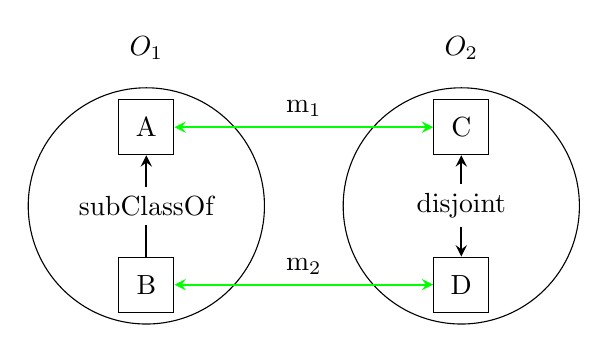
\begin{tikzpicture}
	\node [draw, minimum size = 3cm, align = center,circle] (o1) at (0,0) {};
	\node [draw, minimum size = 3cm, align = center,circle] (o2) at (4,0) {};
	\node [draw, minimum size = 0.7cm, align = center] (A) at (0,1) {A};
	\node [draw, minimum size = 0.7cm, align = center] (B) at (0,-1) {B};
	\node [draw, minimum size = 0.7cm, align = center] (C) at (4,1) {C};
	\node [draw, minimum size = 0.7cm, align = center] (D) at (4,-1) {D};
	\node [align = center, fill = none] (o1l) at (0,2) {$O_1$};
	\node [align = center, fill = none] (o2l) at (4,2) {$O_2$};
	
	\draw[<->,>=stealth,thick,green] (A) to [midway,above] node [align = center, fill=none] {\textcolor{black}{m$_1$}} (C) ;
	\draw[<->,>=stealth,thick,green] (B) to [midway,above] node [align = center, fill=none] {\textcolor{black}{m$_2$}} (D) ;
	\draw[->,>=stealth,thick] (B) to [midway] node [align = center, fill=white] {subClassOf} (A) ;
	\draw[<->,>=stealth,thick] (C) to [midway] node [align = center, fill=white] {disjoint} (D) ;

	\end{tikzpicture}
    \caption{Example of an inconsistent mapping detected by the \textit{Children Metric}. Adopted from \cite{Pathak}}
    \label{fig:cm}
\end{figure}
\subsubsection{Loop detection} \label{loop_detection}
 When merging two ontologies, logical inconsistencies may arise. Given two ontologies $O_1$ and $O_2$ and a mapping $M \subseteq V_{O_1} \times V_{O_2}$, $O_1 \cup O_2$ might contain loops. These loops are logical errors, because they imply that nodes exist which are ancestors and descendants of themselves. In figure ~\ref{fig:loop} an example of such a case can be seen in an abstract representation.

\begin{figure}[h]
    \centering
    	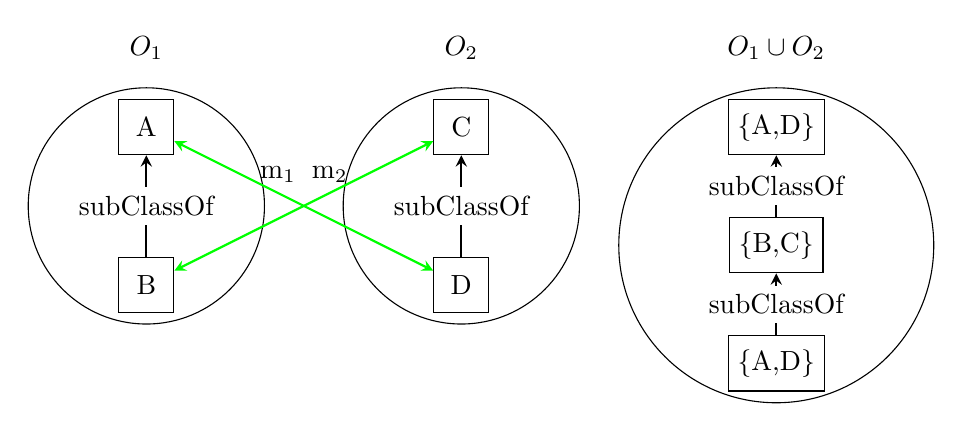
\begin{tikzpicture}
	\node [draw, minimum size = 3cm, align = center,circle] (o1) at (0,0) {};
	\node [draw, minimum size = 3cm, align = center,circle] (o2) at (4,0) {};
	\node [draw, minimum size = 4cm, align = center,circle] (o3) at (8,-0.5) {};
	\node [draw, minimum size = 0.7cm, align = center] (A) at (0,1) {A};
	\node [draw, minimum size = 0.7cm, align = center] (B) at (0,-1) {B};
	\node [draw, minimum size = 0.7cm, align = center] (C) at (4,1) {C};
	\node [draw, minimum size = 0.7cm, align = center] (D) at (4,-1) {D};
	
	\node [draw, minimum size = 0.7cm, align = center] (E) at (8,1) {\{A,D\}};
	\node [draw, minimum size = 0.7cm, align = center] (F) at (8,-0.5) {\{B,C\}};
	\node [draw, minimum size = 0.7cm, align = center] (G) at (8,-2) {\{A,D\}};
	\node [align = center, fill = none] (o1l) at (0,2) {$O_1$};
	\node [align = center, fill = none] (o2l) at (4,2) {$O_2$};
	\node [align = center, fill = none] (o3l) at (8,2) {$O_1 \cup O_2$};
	
	\draw[<->,>=stealth,thick,green] (A) to [pos=0.4,above] node [align = center, fill=none] {\textcolor{black}{m$_1$}} (D) ;
	\draw[<->,>=stealth,thick,green] (B) to [pos=0.6,above] node [align = center, fill=none] {\textcolor{black}{m$_2$}} (C) ;
	\draw[->,>=stealth,thick] (B) to [midway] node [align = center, fill=white] {subClassOf} (A) ;
	\draw[->,>=stealth,thick] (D) to [midway] node [align = center, fill=white] {subClassOf} (C) ;
	\draw[->,>=stealth,thick] (F) to [midway] node [align = center, fill=white] {subClassOf} (E) ;
	\draw[->,>=stealth,thick] (G) to [midway] node [align = center, fill=white] {subClassOf} (F) ;

	\end{tikzpicture}
    \caption{Example of a loop induced by the two matches $m_1$ and $m_2$ during a merge}
    \label{fig:loop}
\end{figure}

In different papers as \cite{Jean-Mary} and \cite{Teymourlouie}, loops where identified as problems, because they are logical errors which imply that there is an error in either one of the two ontologies $O_1$ or $O_2$ or there is at least one wrong match $m \in M$. Additionally, existing loops can break algorithms which are supposed to run on loop free ontologies \cite{Effendi}.

These loops are relevant for this paper, because they indicate that there might be an error in one of the matches. For time constraint reasons, only simple loops between two ontologies induced by exactly two matches are analyzed. In a future work this could be extended.


 The implemented loop check analyzes every match and checks if there is a second match which would induce a loop.
 
 \begin{wrapfigure}{r}{0.5\textwidth}
    \tikzstyle{startstop} = [rectangle, rounded corners, minimum width=3cm, minimum height=1cm,text centered, draw=black, fill=red!30]
    \tikzstyle{io} = [trapezium,trapezium left angle=70, trapezium right angle=110, minimum width=3cm, minimum height=1cm, text centered, draw=black, fill=blue!30]
    \tikzstyle{process} = [rectangle, minimum width=3cm, minimum height=1cm, text centered, draw=black, fill=orange!30]
    \tikzstyle{decision} = [diamond, minimum width=3cm, minimum height=1cm, text centered, draw=black, fill=green!30]
    \tikzstyle{arrow} = [thick,->,>=stealth]
    \centering
    \begin{tikzpicture}[node distance=2cm,scale=0.6, every node/.style={scale=0.8}]
        \node (start) [startstop] {Start};
        \node (in1) [io, below of=start, align = center] {Two ontologies $O_1$, $O_2$\\ in .rdf or .owl format};
        \node (mapFile) [decision, below = 0.5cm of in1,align = center]{mapping file\\ present?};
        \node (fetch) [process,below = 0.5cm of mapFile,align = center]{fetch mappings from BioPortal};
        \node (read) [process, right = 1cm of mapFile,align = center]{read in mappings from file};
        \node (evalMod)[process, below of = fetch,align = center]{create EvaluationModel};
        \node(metric)[process, below of = evalMod,align = center]{calculate metric scores};
        \node(conf)[process, below of = metric,align = center]{calculate confidence score\\ for each existing match};
        \node(out) [io, below of = conf,align = center]{ .csv file with calculated\\ scores of each match};
        \node (end)[startstop,below of =out]{Stop};
        %\node (pro1) [process, below of=in1] {Process 1};
        \draw [arrow] (start) -- (in1);
        \draw [arrow] (in1) -- (mapFile);
        \draw [arrow] (mapFile) -- node[midway,left] {no} (fetch);
        \draw [arrow] (mapFile) -- node[midway, above] {yes} (read);
        \draw [arrow] (fetch) -- (evalMod);
        \draw [arrow] (read) |- (evalMod);
        \draw [arrow] (evalMod) -- (metric);
        \draw [arrow] (metric) -- (conf);
        \draw [arrow] (conf) -- (out);
        \draw [arrow] (out) -- (end);
    \end{tikzpicture}
    \caption{Flowchart of the program flow of our implementation}
    \label{fig:wf}
    \vspace{-85pt}
\end{wrapfigure}
 
 Given a match $(a,b) \in M$, it is checked if there exists a match between an ancestor of $a$ and a descendant of $b$ and vice versa. If this is the case, there exists a loop in $O_1 \cup O_2$.

\section{Experiment} \label{experiment}

In order to evaluate the quality of existing mappings in BioPortal, we implemented the metrics presented in the previous section and compared the results against the silver standard from Pistoia.

\subsection{Implementation} \label{implementation}

We implemented our approach in Java, since it provides useful libraries to work with ontologies, such as \textit{Apache Jena}\footnote{https://jena.apache.org/}. The workflow of our implementation is illustrated in figure ~\ref{fig:wf}. First the user needs to provide two ontologies $O_1$ and $O_2$ in $.rdf$ or $.owl$ format, which are read in and represented as an instance of the OntModel class provided by \textit{Apache Jena}. If the user also provides a mapping file, which is a text file with two columns, where each column represents the URI of a class in $O_1$ and $O_2$ respectively, the file is also read in. If no such file is present, we fetch the mappings from the BioPortal, using the REST API\footnote{http://data.bioontology.org/documentation}. When we gathered all the data, we create an instance of EvaluationModel. The EvaluationModel class provides the necessary datastructures to store all the calculated metric scores for each match. After that, we calculate for each match the scores for the different metrics presented in the previous section. 

Based on the results of the metric scores we calculate a confidence score between 2 and 4, similar to the silver standard. The confidence score is based on a "naive" decision tree, which is illustrated in figure ~\ref{fig:dt}. The decision tree uses "intuitive" rules to calculate a score. First, we check if the mapping contains a loop. If this is the case, the probability is high that the match is bad, thus we assing in this case the score 2. If it does not contain a loop, we check the result of the \textit{Children Metric}. If the result is true, we take the minimum of the calculated similarity metrics for the labels and compare if it is under the threshold of $0.8$. If it is, we set the score to 2, otherwise to 3. In the case, where the result of the \textit{Children Metric} is false, we do the same but set the score to 3 if the result is under $0.8$ and to 4 otherwise. Finally, we output a $.csv$ file, which contains all results we calculated. For each match we output the URIs of the classes in $O_1$ and $O_2$, and the calculated metric results and our calculated score. The implementation and details can be found in the git repository (\href{https://git.rwth-aachen.de/tobias.raewer/kglab-project}{https://git.rwth-aachen.de/tobias.raewer/kglab-project}).

\begin{figure}[!h]
    \centering
    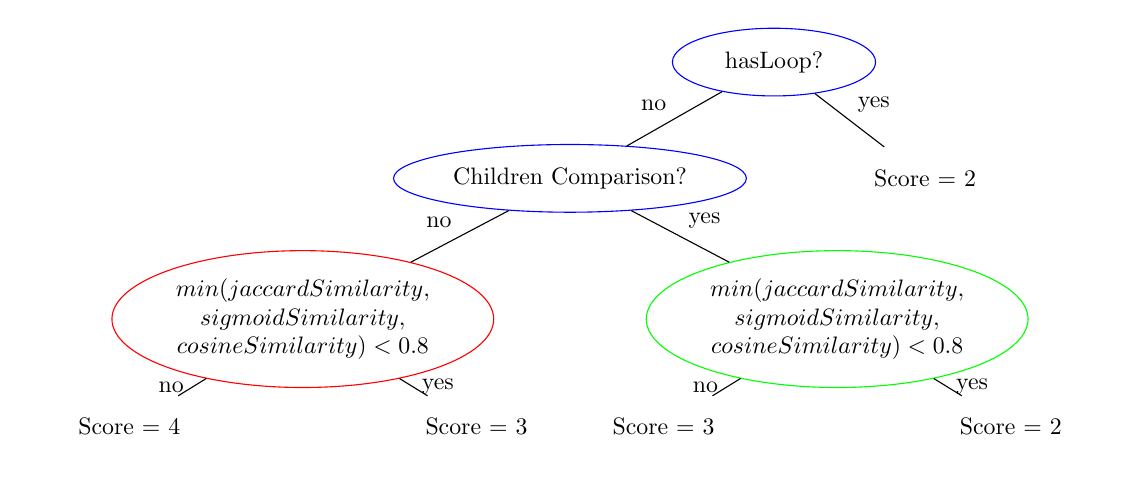
\begin{tikzpicture}[scale = 0.86,transform shape]
    \tikzstyle{n} = [ellipse, minimum width=3cm, minimum height=1cm,text centered, draw=blue]
    \tikzstyle{arrow} = [thick,->,>=stealth]
        \node (hl) [n] {hasLoop?};
        \node (hc) [n,below left= 1cm and 0.1cm of hl] {Children Comparison?};
        \node (s1) [n,below right = 1cm and 0.1cm of hl, draw = none] {Score = 2};
        \node (min1)[n,below left= 1cm and 0.1cm of hc,align = center,draw = red]{$min(jaccardSimilarity,$\\ $sigmoidSimilarity,$\\ $cosineSimilarity) < 0.8$};
        \node (min2)[n,below right= 1cm and 0.1cm of hc,align = center,draw = green]{$min(jaccardSimilarity,$\\ $sigmoidSimilarity,$\\ $cosineSimilarity) < 0.8$};
        \node (s2) [n,below right=0.5cm and -0.5cm of min2, draw = none] {Score = 2};
        \node (s3) [n,below left= 0.5cm and -0.5cm  of min2, draw = none] {Score = 3};
        \node (s4) [n,below right=0.5cm and -0.5cm of min1, draw = none] {Score = 3};
        \node (s5) [n,below left=0.5cm and -0.5cm of min1, draw = none] {Score = 4};
        \draw (hl) -- node[midway,above left]{no} (hc);
        \draw (hl) -- node[midway,above right]{yes}(s1);
        \draw (hc) --node[midway,above left]{no} (min1);
        \draw (hc) --node[midway,above right]{yes} (min2);
        \draw (min2) -- node[right]{yes}(s2);
        \draw (min2) -- node[left]{no}(s3);
        \draw (min1) -- node[right]{yes}(s4);
        \draw (min1) -- node[left]{no}(s5);
    \end{tikzpicture}
    \caption{Intuitive decision tree to calculate the confidence score of the quality of a match}
    \label{fig:dt}
\end{figure}

\begin{table}[H]
\centering
\caption{Ontologies used for evaluation}\label{onts}
\begin{tabular}{|c|c|c|}
\hline
    \textbf{Ontology}&
    \textbf{Acronym}&
    \textbf{\# Classes}
\\
\hline
 Human Phenotype Ontology & HP & 18,154 \\
\hline
 Mammalian Phenotype Ontology & MP & 14,028 \\
\hline
\end{tabular}
\end{table}
\subsection{Evaluation} \label{evaluation}
To evaluate our results, we use the $.csv$ file given as output of our program. We compared our results against the provided scores by the silver standard of Pistoia. Since they provided the scores for mappings between the Human Phenotype Ontology (HP) and the Mammalian Phenotype Ontology (MP), we also used these two ontologies in our evaluation (cf. Table \ref{onts}). We downloaded the latest version of both ontologies in $.xrdf$ format from the BioPortal website \footnote{https://BioPortal.bioontology.org/}. To retrieve our results, we ran our implementation twice. In the first run, we only used the mappings we retrieved from BioPortal using the REST API. In the second run, we provided a mapping file, which contains all the mappings, we have a score from the silver standard (cf. Table \ref{maps}). 

\begin{table}[H]
\centering
\caption{Number of retrieved mappings}\label{maps}
\begin{tabular}{|c|c|c|}
\hline
    \textbf{Ontology Pair}&
    \textbf{Retrieved Mappings (REST API)}&
    \textbf{Mappings (Silver Standard)}
\\
\hline
 HP-MP & 750 & 2005 \\
 \hline
\end{tabular}
\end{table}
After obtaining the results of both runs, we used a Jupyter Notebook to also compare our "naive" score against machine learning techniques.  We created two models, to predict the score based on our metric scores. One which uses a multinomial logistic regression estimator, and one which uses a random forest estimator. Therefore, we used the silver standard as ground truth and split the data into a test set and a training set. The test set contains 40\% of the data. General statistics of the sets can be found in Table \ref{ml}.
\begin{table}[H]
\centering
\caption{Statistics of test sets used for evaluation}\label{ml}
\begin{tabular}{|c|c|p{1.5cm}|p{1.5cm}|p{1.5cm}|}
\hline
    \textbf{Approach}&
    \textbf{\#Mappings}&
    \multicolumn{3}{|c|}{\textbf{Scores (silver standard)}}\\
    \hline
    & & \hfil \textbf{2} & \hfil \textbf{3} & \hfil \textbf{4}\\
    \hline
    Naive (REST API) & 557 & \hfil 28 & \hfil 7 & \hfil 522\\
    \hline
    Logistic regression (REST API) & 223 & \hfil 12 & \hfil 4 & \hfil 207\\
    \hline
    Random forest (REST API) & 223 & \hfil 12 & \hfil 4 & \hfil 207\\
    \hline
    Naive (Mapping file) & 2005 & \hfil 406 & \hfil 248 & \hfil 1351\\
    \hline
    Logistic regression (Mapping file) & 802 & \hfil 174 & \hfil 93 & \hfil 535\\
    \hline
    Random forest (Mapping file) & 802 & \hfil 174 & \hfil 93 & \hfil 535\\
    \hline

\end{tabular}
\end{table}

The results after estimating the scores with the machine learning techniques and comparing our "naive" scores against the silver mapping scores are shown in Table \ref{res}.

\begin{table}[H]
\centering
\caption{Results of our evaluation}\label{res}
\begin{tabular}{|c|c|c|c|}
\hline
    \textbf{Approach}&
    \textbf{Precision}&
    \textbf{Recall}&
    \textbf{F1-measure}\\
    \hline
    Naive (REST API) & 0.88389 & 0.88509 & 0.88352 \\
    \hline
    Logistic regression (REST API) & 0.86165 & 0.92825 & 0.89371 \\
    \hline
    Random forest (REST API) & 0.90198 & 0.91479 & 0.90835 \\
    \hline
    Naive (Mapping file) & 0.66276 & 0.49027 & 0.52989 \\
    \hline
    Logistic regression (Mapping file) & 0.61291 & 0.69576 & 0.62828 \\
    \hline
    Random forest (Mapping file) & 0.66611 & 0.71321 & 0.66593 \\
    \hline

\end{tabular}
\end{table}

As one can see, our predictions of the scores for quality of a match using the mappings obtained by the REST API seem to be very good. All three approaches reach nearly a F1-measure of 90\%, where the random forest approach seems to be the best approach with a precision of 90.198\% and a F1-score of 90.835\%. However, if we take a look at Figure \ref{fig:tp}, we see that these numbers have to be interpreted very carefully. The data set we are using for our evaluation using the REST API contains mostly matching with the score 4. We only have 28 matches with score 2 and 7 matches with score 3. This is not enough data to train the machine learning estimators sufficiently. As one can see, the linear regression model predicts all matches with score 4 correctly, but none with the score 2 or 3. Nevertheless, it reaches a F1-measure of nearly 90\%.\\

    
Considering the mappings we measured using the mapping file, we see that the scores decrease. Our naive approach reaches only an F1-measure of 52.989\%. We predicted 58.11\% of the score 4, 58.47\% of score 3, and 13.05\% correctly. With the machine learning approaches the results improve, where the random forest approach gives us the best results. We reach a precision of 66.611\% and a F1-measure of 66.593\%. Furthermore, we see that the predictions for score 4 are very good with 94.21\% (cf. Figure \ref{fig:tp}). However, the predictions for score 3 are only 9.677\%, which is not very good.
Nevertheless, it is important to mention that also this test set is relatively small and the scores in the silver standard are provided by domain experts. They might know things about matchings, which our approach currently does not consider and therefore it is hard to estimate the quality of a match.
 
\section{Conclusion and Future Work} \label{conclusion}
In this project we have developed a framework, for measuring the quality of existing mappings between two ontologies. Our approach considers several metrics to assess the quality based on lexical similarity and structural similarities and finally give an estimation how good the quality of a match is by providing a score. This score is calculated by an ``naive" approach and two different machine learning techniques. Then, we have performed a evaluation of our proposal, to see how our metrics perform. Therefore, we evaluated the mapping quality between the Human Phenotype Ontology and the Mammalian Phenotype Ontology, and used the silver standard provided by Pistoia as reference data and ground truth. 
Our results seem to be very good, if we consider mostly matches based on lexical similarity (e.g. found by the LOOM algorithm). In this case we get for all three approaches a F1-measure of nearly 90\%. However, if we increase to number of mappings and also provide mappings, which are not present in BioPortal, the score decreases. In this case, we get the best results with the random forest machine learning approach, with a F1-measure of about 67\%. \\
    \begin{figure}[H]
        \begin{subfigure}{.5\textwidth}
            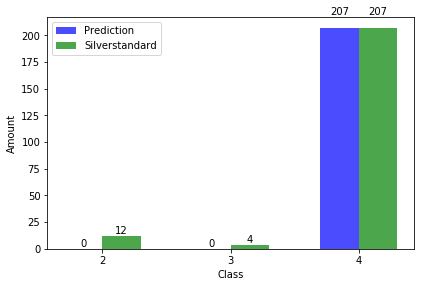
\includegraphics[scale=0.35]{lrREST.png}
            \caption{TP of linear regression model using REST API}
        \end{subfigure}
        \begin{subfigure}{.4\textwidth}
            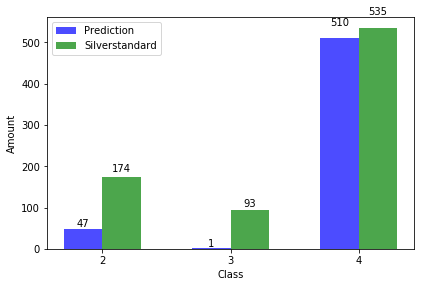
\includegraphics[scale=0.35]{lrFile.png}
            \caption{TP of linear regression model using map file}
        \end{subfigure}
        \\
        \begin{subfigure}{.5\textwidth}
            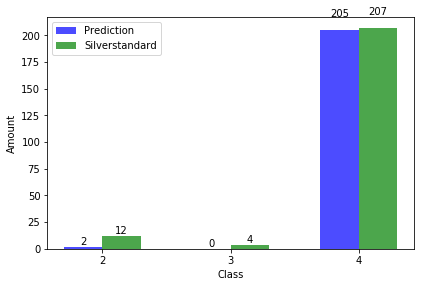
\includegraphics[scale=0.35]{rfREST.png}
            \caption{TP of random forest model using REST API}
        \end{subfigure}
        \begin{subfigure}{.4\textwidth}
            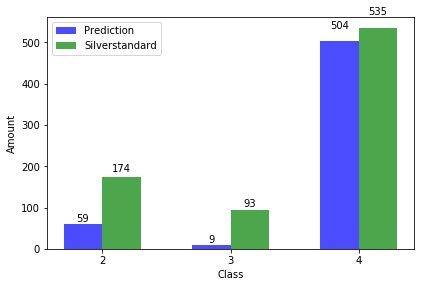
\includegraphics[scale=0.35]{rfFile.png}
            \caption{TP of random forest model using map file}
        \end{subfigure}
        \\
        \begin{subfigure}{.5\textwidth}
            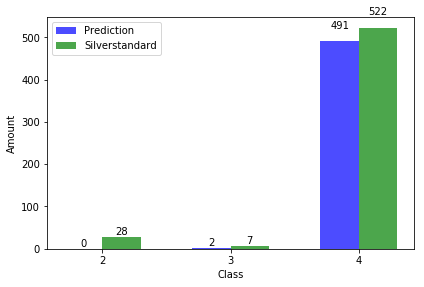
\includegraphics[scale=0.35]{nREST.png}
            \caption{TP of naive model using REST API}
        \end{subfigure}
        \begin{subfigure}{.4\textwidth}
            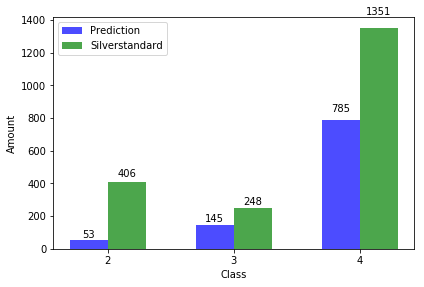
\includegraphics[scale=0.35]{nFile.png}
            \caption{TP of naive model using map file}
        \end{subfigure}
        \caption{True Positives (TP) of different approaches prediction the quality of a match}
        \label{fig:tp}
    \end{figure}
    
Considering these results, we can say that our approach is able to assess the quality of mappings between two ontologies, especially if these matchings are based on lexical similarity. However, we have to admit that there is still a lot room for improvement. Therefore, we want to extend our framework in the future to also support metrics based on semantics to get better results. Furthermore, we aim to provide a framework which does not only consider two ontologies, but multiple. However, it is still hard to evaluate the quality of mappings between ontologies, because there are very few reference data sets, which provide a standard for the quality of matches. Therefore, it is also a goal in the future to provide such a reference data set.

\subsection{Personal conclusions} \label{personal_conclusions}
\subsubsection{Personal conclusion Tobias}
The main part I contributed to the project, was the handling of the information we retrieved from the ontologies ,i.e., how to use the REST API and later on, when we decided to use ontology files, to adapt our code to work with the \textit{Apache Jena} library. Furthermore, I did research on the Children Metric and implemented it. Finally, I also evaluated the data we retrieved as output from our program.
During the project, I have learned a lot about the structuring of data in an ontology, how it is represented in a file, and how we can access the information in it. Furthermore, one thing I learned is that handling such big amounts of data is really difficult, especially if data is not complete and only present in different formats.
\subsubsection{Personal conclusion Lina} Primarily, I contributed to applying lexical similarity metrics to the different properties.  Also, I focused on the data handling when required, specially when retrieving properties from the ontology classes. In the initial phase of the project, I contributed with the problem definition and proposed solution, alongside with my colleagues. I also contributed to the literature research, specially with respect to the metrics. Finally, I contributed with the documentation during the meetings, as well as the writing of this report. I learnt a lot about the practical aspect of knowledge graphs (KG) and how to technically interact with them. Also, I learnt about information retrieval in the context of ontologies and KG, and the evaluation of results.
\subsubsection{Personal conclusion Jonas}
My main contributions to the code base were focused on the loop detection, the application
of the similarity metrics to subgraphs, the modelling of the data and development of helper functions
whose need arose during development. Additionally, I spent time on literature research,
mainly focusing on mapping evaluation and loop detection, and on the documentation of our progress.
I learned  a lot about knowledge graphs and ontologies in particular, and also realized
that the application of the theory to practice is not always as easy as expected. For instance,
there is nearly never an exact truth, but only different approximations, which makes
the evaluation of your results much more difficult. 


%
% ---- Bibliography ----
%
% BibTeX users should specify bibliography style 'splncs04'.
% References will then be sorted and formatted in the correct style.
%
% \bibliographystyle{splncs04}
% \bibliography{mybibliography}
%
\begin{thebibliography}{8}

\bibitem{Noy}
Noy, N., Mcguinness, D.: Ontology Development 101: A Guide to Creating Your First Ontology. Stanford University (2001)

\bibitem{Kalfoglou}
Kalfoglou, Y., Schorlemmer, M.: Ontology Mapping: The State of the Art. Knowl. Eng. Rev.\textbf{18}(1), 1--31 (2003)

\bibitem{BioPortal}
Whetzel PL, Noy NF, Shah NH, Alexander PR, Nyulas C, Tudorache T, Musen MA. BioPortal: enhanced functionality via new Web services from the National Center for Biomedical Ontology to access and use ontologies in software applications. Nucleic Acids Res. 2011 Jul;39(Web Server issue):W541-5. Epub 2011 Jun 14.

\bibitem{ref_url1}
BioPorltal - NCBO Wiki, \url{https://www.bioontology.org/wiki/BioPortal_Help}. Last accesed 04 Aug 2019

\bibitem{ref_url2}
Stanford Knowledge Systems - AI Laboratory - What is an Ontology?, \url{http://www-ksl.stanford.edu/kst/what-is-an-ontology.html}. Last accessed 27 Jul 2019

\bibitem{ref_url3}
Modulo 5.2 Ontology Matching - Knowledge and Data VU Amsterdam, \url{https://www.youtube.com/watch?v=gnq9I0OTjRo\&t=920s}. Last accessed 27 Jul 2019

\bibitem{Hooi}
Hooi Y.K., Hassan M.F., Shariff A.M.: A Survey on Ontology Mapping Techniques. In: Jeong H., S. Obaidat M., Yen N., Park J. (eds.) Advances in Computer Science and its Applications 2014, Lecture Notes in Electrical Engineering, vol. 279.
Springer, Berlin, Heidelberg (2014). \doi{10.1007/978-3-642-41674-3\_118}

\bibitem{Euzenat}
Euzenat, J., Shvaiko, P.: Ontology Matching. 2nd edn. Springer Publishing Company, Incorporated (2013)

\bibitem{Heflin}
Heflin, J., Song, D.: Ontology Instance Linking: Towards Interlinked Knowledge Graphs. In: Proceedings of the Thirtieth AAAI Conference on Artificial Intelligence, pp. 4163--4169. AAAI Press, Phoenix, Arizona (2016)

\bibitem{Shvaiko}
Shvaiko, P., Euzenat, J.: Ten Challenges for Ontology Matching. In: Proceedings of the OTM 2008 Confederated International Conferences, CoopIS, DOA, GADA, IS, and ODBASE 2008. Part II on On the Move to Meaningful Internet Systems, pp. 1164--1182. Springer-Verlag, Monterrey, Mexico (2008)

\bibitem{Saveta}
Saveta, T., Daskalaki, E., Flouris, G., Fundulaki, I., Herschel, M., Ngonga Ngomo, A.: Pushing the Limits of Instance Matching Systems: A Semantics-Aware Benchmark for Linked Data. In: Proceedings of the 24th International Conference on World Wide Web, pp. 105--106. ACM, Florence, Italy (2015)

\bibitem{Euzenat2}
Euzenat, J.: Semantic Precision and Recall for Ontology Alignment Evaluation. In: Proceedings of the 20th International Joint Conference on Artificial Intelligence, pp. 348--353. Morgan Kaufmann Publishers Inc., Hyderabad, India (2007)

\bibitem{ref_url4}
Jaccard Coefficient - an overview, \url{https://www.sciencedirect.com/topics/computer-science/jaccard-coefficient}. Last accessed 04 Aug 2019

\bibitem{Likavec}
Likavec, S., Lombardi, I., Cena, F.: How to improve Jaccard’s feature-based similarity measure. In: Semantic Web Journal (2017)

\bibitem{Oliveira}
Oliveira, D., Butt, A., Haller, A., Rebholz-Schuhmann, D., Sahay, R.: Where to search top-K biomedical ontologies?. In: Briefings in Bioinformatics. (2018)

\bibitem{Pathak}
Pathak, J., Chute, C.: Debugging mappings between biomedical ontologies: Preliminary results from the NCBO BioPortal mapping repository. In: ICBO, pp. 95. Citeseer, (2009)

\bibitem{Jean-Mary}
Jean-Mary YR, Shironoshita EP, Kabuka MR: Ontology Matching with Semantic Verification. In: Web Semant. 2009;7(3):235–251. (2009)

\bibitem{Effendi}
Y. A. Effendi, R. Sarno: SWRL rules for identifying short loops in business process ontology model. In: 2017 11th International Conference on Information \& Communication Technology and System (ICTS), Surabaya, 2017, pp. 209-214. (2017)

\bibitem{Teymourlouie}
Mehdi Teymourlouie, Ahmad Zaeri, Mohammadali Nematbakhsh, Matthias Thimm, Steffen Staab. Detecting hidden errors in an ontology using contextual knowledge. In: Expert Systems with Applications, Volume 95, 2018, Pages 312-323. (2018)


\bibitem{Achichi}
Achichi, M., Cheatham, M., Dragisic, Z., Euzenat, J., Faria, D., Ferrara, A., Flouris, G., Fundulaki, I., Harrow, I., Ivanova, V., Jim{\'e}nez-Ruiz, E., Kolthoff, K., Kuss, E., Lambrix, P., Leopold, H., Li, H., Meilicke, C., Mohammadi, M., Montanelli, S., Pesquita, C., Saveta, T., Shvaiko, P., Splendiani, A., Stuckenschmidt, H., Thi{\'e}blin, {\'E}., Todorov, K., Trojahn dos Santos, C., Zamazal, O.: Results of the Ontology Alignment Evaluation Initiative 2017. In:  OM: Ontology Matching (CEUR Workshop Proceedings), pp. 61-113., Wien, Austria (2017)

\bibitem{Harrow}
Harrow, I., Jim{\'e}nez-Ruiz, E., Splendiani, A., Romacker, M., Woollard, P., Markel, S., Alam-Faruque, Y., Koch, M., Malone, J., Waaler, A.: Matching disease and phenotype ontologies in the ontology alignment evaluation initiative. In: J. Biomedical Semantics, pp. 55.BioMed Central, (2017)

\bibitem{Fleischhacker}
Fleischhacker, D., Stuckenschmidt, H., A.: A Practical Implementation of Semantic Precision and Recall. In: 2010 International Conference on Complex, Intelligent and Software Intensive Systems, pp. 986-991.(2010)

\bibitem{Amith}
Amith, M., He, Z., Bian, J., Lossio-Ventura, J. A., Tao, C.: Assessing the practice of biomedical ontology evaluation: Gaps and opportunitiesy. In: Journal of biomedical informatics, pp. 1–13. (2018)

\bibitem{Todorov}
Todorov, K., Geibel, P., K\"{u}hnberger, K.: Mining Concept Similarities for Heterogeneous Ontologies. In: Proceedings of the 10th Industrial Conference on Advances in Data Mining: Applications and Theoretical Aspects, pp. 86--100. Springer-Verlag, Berlin, Germany. (2010)

\end{thebibliography}
\end{document}
